% !TeX root = ../arara-manual.tex
\chapter{Building from source}
\label{chap:buildingfromsource}

\arara\ is a Java application licensed under the \href{http://www.opensource.org/licenses/bsd-license.php}{New BSD License}, a verified GPL-compatible free software license, and the source code is available in the project repository at \href{https://github.com/cereda/arara}{GitHub}. This chapter provides detailed instructions on how to build our tool from source.

\section{Requirements}
\label{sec:requirements}

In order to build our tool from source, we need to ensure that our development environment has the minimum requirements for a proper compilation. Make sure the following items are contemplated:

\begin{itemize}[label={\cbyes{-2}}]
\item On account of our project being hosted at \href{https://github.com}{GitHub}, an online source code repository, we highly recommend the installation of \rbox{git}, a version control system for tracking changes in computer files and coordinating work on those files among multiple people. Alternatively, you can directly obtain the source code by requesting a \href{https://github.com/cereda/arara/archive/master.zip}{source code download} in the repository. In order to check if \rbox{git} is available in your operating system, run the following command in the terminal (version numbers might vary):

\begin{codebox}{Terminal}{teal}{\icnote}{white}
$ git --version
git version 2.17.1
\end{codebox}

Please refer to \href{https://git-scm.com/}{project website} in order to obtain specific installation instructions for your operating system. In general, most recent Unix systems have \rbox{git} installed out of the shelf.

\item Our tool is written in the Java programming language, so we need a proper Java Development Kit,  a collection of programming tools for the Java platform. Our source code is known to be compliant with several vendors, including Oracle, OpenJDK, and Azul Systems. In order to check if your operating system has the proper tools, run the following command in the terminal (version numbers might vary):

\begin{codebox}{Terminal}{teal}{\icnote}{white}
$ javac -version
javac 1.8.0_171
\end{codebox}

The previous command, as the name suggests, refers to the \rbox{javac} tool, which is the Java compiler itself. The most common Java Development Kit out there is from \href{http://www.oracle.com/technetwork/java/javase/downloads/index.html}{Oracle}. However, several Linux distributions (as well as some developers, yours truly included) favour the OpenJDK vendor, so your milleage may vary. Please refer to the corresponding website of the vendor of your choice in order to obtain specific installation instructions for your operating system.

\item As a means to provide a straightforward and simplified compilation workflow, \arara\ relies on Apache Maven, a software project management and comprehension tool. Based on the concept of a project object model, Maven can manage builds, reporting and documentation from a central piece of information. In order to check if \rbox{mvn}, the Maven binary, is available in your operating system, run the following command in the terminal (version numbers might vary):

\begin{codebox}{Terminal}{teal}{\icnote}{white}
$ mvn --version
Apache Maven 3.5.2 (Red Hat 3.5.2-5)
Maven home: /usr/share/maven
Java version: 1.8.0_171, vendor: Oracle Corporation
Java home: /usr/lib/jvm/java-1.8.0-openjdk-
    1.8.0.171-4.b10.fc28.x86_64/jre
Default locale: pt_BR, platform encoding: UTF-8
OS name: "linux", version: "4.16.16-300.fc28.x86_64",
    arch: "amd64", family: "unix"
\end{codebox}

Please refer to \href{https://maven.apache.org/}{project website} in order to obtain specific installation instructions for your operating system. In general, most recent Linux distributions have the Maven binary, as well the proper associated dependencies, available in their corresponding repositories.

\item For a proper repository cloning, as well as the first Maven build, an active Internet connection is required. In particular, Maven dynamically downloads Java libraries and plug-ins from one or more online repositories and stores them in a local cache. Be mindful that subsequent builds can occur offline, provided that the local Maven cache exists.
\end{itemize}

\arara\ can be easily built from source, provided that the aforementioned requirements are contemplated. The next section presents the compilation details, from repository cloning to a proper Java archive generation.

\begin{messagebox}{One tool to rule them all}{araracolour}{\icok}{white}
\setlength{\parskip}{1em}
For the brave, there is the \href{https://sdkman.io/}{Software Development Kit Manager}, an interesting tool for managing parallel versions of multiple software development kits on most Unix based systems. In particular, this tool provides out of the shelf support for several Java Development Kit vendors and versions, as well as most recent versions Apache Maven.

Personally, I prefer the packaged versions provided by my favourite Linux distribution (Fedora), but this tool is a very interesting alternative to set up a development environment with little to no effort.
\end{messagebox}

\section{Compiling the tool}
\label{sec:compilingthetool}

First and foremost, we need to clone the project repository into our development environment, so we can build our tool from source. Run the following command in the terminal:

\begin{codebox}{Terminal}{teal}{\icnote}{white}
$ git clone https://github.com/cereda/arara
\end{codebox}

Wait a couple of seconds (or minutes, depending on your Internet connection) while the previous command clones the project repository hosted at GitHub into a directory named \abox[araracolour]{arara/} within the working directory. Be mindful that this operation pulls down every version of every file for the history of the project. Fortunately, the version control system has the notion of a \emph{shallow clone}, which is a more succinctly meaningful way of describing a local repository with history truncated to a particular depth during the clone operation. If you want to get only the latest revision of everything in our repository, run the following command in the terminal:

\begin{codebox}{Terminal}{teal}{\icnote}{white}
$ git clone https://github.com/cereda/arara --depth 1
\end{codebox}

This operation is way faster than the previous one, for obvious reasons. Unix terminals typically start at \abox[araracolour]{USER\_HOME} as working directory, so the newly cloned \abox[araracolour]{arara/} directory is almost certain to be accessible from that level. Now, we need to navigate to a directory named \abox[araracolour]{application/} inside our project structure, where the source code and the corresponding build file are located. Run the following command in the terminal:

\begin{codebox}{Terminal}{teal}{\icnote}{white}
$ cd arara/application
\end{codebox}

The previous command should take us inside the \abox[araracolour]{application/} directory of our project, where the source code and the corresponding build file are located. Let us make sure we are in the correct location by running the following command in the terminal:

\begin{codebox}{Terminal}{teal}{\icnote}{white}
$ ls
pom.xml  src
\end{codebox}

Great, we are in the correct location! From the previous output, let us inspect the directory contents. The \abox[araracolour]{src/} directory, as the name suggests, contains the source code organized in an established package structure, whereas \rbox{pom.xml} is the corresponding build file written in the Project Object Model format, a special XML file that contains information about the project and configuration details used by Apache Maven to build the project. In order to build our tool, run the following command in the terminal:

\begin{codebox}{Terminal}{teal}{\icnote}{white}
$ mvn compile assembly:single
\end{codebox}

Apache Maven is based around the central concept of a build life cycle. The \rbox{compile} phase, as the name suggests, compiles the source code of the project using the underlying Java compiler. From the previous command, bound to this particular build phase, note that there is an \rbox{assembly:single} plug-in goal which aggregates the project output along with its dependencies and other files into a single distributable archive. An \emph{assembly} is a group of files, directories and dependencies that are assembled into an archive format and distributed. In our case, the resulting file will be a typical Java archive file, with the \rbox{jar} extension. The first Maven build will take a couple of seconds (or minutes, depending on your Internet connection), as the tool will download all dependencies and required plug-ins for proper compilation and packaging. Subsequent builds will be significantly faster. Finally, after some time, Maven will output the following message as result (please note that the entire compilation and packaging only took 10 seconds on my development machine due to an existing local cache):

\begin{codebox}{Terminal}{teal}{\icnote}{white}
[INFO] ---------------------------------------------------------
[INFO] BUILD SUCCESS
[INFO] ---------------------------------------------------------
[INFO] Total time: 10.371 s
[INFO] Finished at: 2018-06-22T18:38:02-03:00
[INFO] Final Memory: 39M/184M
[INFO] ---------------------------------------------------------
\end{codebox}

On account of a successful build in our previous interaction, there is now a newly created \abox[araracolour]{target/} directory containing compiled classes, a established package structure and, at last but not least, our assembly. Now, let us move the resulting Java archive file from that particular directory to \abox[araracolour]{application/} which is our current directory. It is important to note that the aforementioned assembly plug-in adds the \rbox{jar-with-dependencies} reference to the file name in order to differentiate a proper assembly from a typical Java archive file. Run the following command in the terminal (please note that the Java archive file was also renamed during the move operation):

\begin{codebox}{Terminal}{teal}{\icnote}{white}
$ mv target/arara-4.0-jar-with-dependencies.jar arara.jar
\end{codebox}

% TODO fix reference
Now, our current directory contains the final \rbox{arara.jar} Java archive file properly built from source. This file can be safely distributed and deployed, as seen later on in Section~\ref{foo}, on page~\pageref{foo}. You can also test the resulting file by running the following command in the terminal:

\begin{codebox}{Terminal}{teal}{\icnote}{white}
$ java -jar arara.jar
  __ _ _ __ __ _ _ __ __ _ 
 / _` | '__/ _` | '__/ _` |
| (_| | | | (_| | | | (_| |
 \__,_|_|  \__,_|_|  \__,_|

arara 4.0 (revision 1)
Copyright (c) 2012-2018, Paulo Roberto Massa Cereda
All rights reserved

usage: arara [file [--dry-run] [--log] [--verbose | --silent]
             [--timeout N] [--max-loops N] [--language L]
             [ --preamble P ] [--header] | --help | --version]
 -h,--help                 print the help message
 -H,--header               extract directives only in the file header
 -l,--log                  generate a log output
 -L,--language <code>      set the application language
 -m,--max-loops <number>   set the maximum number of loops
 -n,--dry-run              go through all the motions of running a
                           command, but with no actual calls
 -p,--preamble <name>      set the file preamble based on the
                           configuration file
 -s,--silent               hide the command output
 -t,--timeout <number>     set the execution timeout (in milliseconds)
 -V,--version              print the application version
 -v,--verbose              print the command output
\end{codebox}

The following optional Maven phase is used to handle the project cleaning, including the complete removal of the \abox[araracolour]{target/} directory. As a result, the project is then restored to the initial state without any generated Java bytecode. Run the following command in the terminal:

\begin{codebox}{Terminal}{teal}{\icnote}{white}
$ mvn clean
\end{codebox}

This section covered the compilation details for building \arara\ from source. The aforementioned steps are straightforward and can be automated in order to generate snapshots and daily builds. Happy compilation!

\begin{messagebox}{While you wait\ldots}{araracolour}{\icok}{white}
\begin{minipage}{0.5\textwidth}
The first Maven build can take several minutes, depending on your Internet connection. While you wait, have a cup of coffee, plant a tree, write a letter, talk to a friend, help an elder, sing, whistle, eat chocolate, spend time with your parents, read a book, exercise, hug your pet, watch the sunrise, smile, have an ice cream, laugh, be friendly. Always make a difference, my friend. Life goes by in a blink of an eye!
\end{minipage}\hspace{1em}
\begin{minipage}{0.45\textwidth}
\vspace{.8em}
{\centering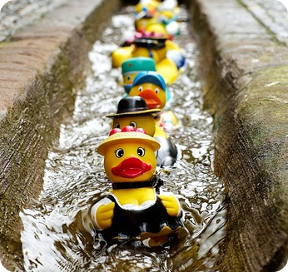
\includegraphics[width=0.9\textwidth]{figures/ducks.png}\par}
\vspace{.8em}
\end{minipage}
\end{messagebox}
